\documentclass[a4paper,UKenglish,cleveref, autoref, thm-restate]{oasics-v2019}
%This is a template for producing OASIcs articles. 
%See oasics-manual.pdf for further information.
%for A4 paper format use option "a4paper", for US-letter use option "letterpaper"
%for british hyphenation rules use option "UKenglish", for american hyphenation rules use option "USenglish"
%for section-numbered lemmas etc., use "numberwithinsect"
%for enabling cleveref support, use "cleveref"
%for enabling autoref support, use "autoref"
%for anonymousing the authors (e.g. for double-blind review), add "anonymous"
%for enabling thm-restate support, use "thm-restate"

%\graphicspath{{./graphics/}}%helpful if your graphic files are in another directory

\usepackage{tikz}
\usepackage{forest}
\usepackage{behaviortrees}
\usepackage{float}

\bibliographystyle{plainurl}% the mandatory bibstyle

\def\bht{BhTSL}
\title{\bht, Behavior Trees Specification and Processing} %TODO Please add

\titlerunning{\bht, Behavior Trees} %TODO optional, please use if title is longer than one line

\author{Miguel Oliveira}{Centro ALGORITMI, DI, Universidade do Minho, Portugal}{}{}{}
\author{Pedro Mimoso Silva}{Centro ALGORITMI, DI, Universidade do Minho, Portugal}{}{}{}
\author{Pedro Moura}{Centro ALGORITMI, DI, Universidade do Minho, Portugal}{}{}{}
\author{José João Almeida}{Centro ALGORITMI, DI, Universidade do Minho, Portugal}{}{}{}
\author{Pedro Rangel Henriques}{Centro ALGORITMI, DI, Universidade do Minho, Portugal}{}{}{}


\authorrunning{M. Oliveira et al.} %TODO mandatory. First: Use abbreviated first/middle names. Second (only in severe cases): Use first author plus 'et al.'

\Copyright{John Q. Public and Joan R. Public} %TODO mandatory, please use full first names. OASIcs license is "CC-BY";  http://creativecommons.org/licenses/by/3.0/

\ccsdesc[100]{\textcolor{red}{Replace ccsdesc macro with valid one}} %TODO mandatory: Please choose ACM 2012 classifications from https://dl.acm.org/ccs/ccs_flat.cfm 

\keywords{Game development, Behavior trees (BT), DSL, NPC, Code generation} %TODO mandatory; please add comma-separated list of keywords

\acknowledgements{I want to thank \dots}%optional

%\nolinenumbers %uncomment to disable line numbering

%\hideOASIcs  %uncomment to remove references to OASIcs series (logo, DOI, ...), e.g. when preparing a pre-final version to be uploaded to arXiv or another public repository

%Editor-only macros:: begin (do not touch as author)%%%%%%%%%%%%%%%%%%%%%%%%%%%%%%%%%%
\EventEditors{John Q. Open and Joan R. Access}
\EventNoEds{2}
\EventLongTitle{42nd Conference on Very Important Topics (CVIT 2016)}
\EventShortTitle{CVIT 2016}
\EventAcronym{CVIT}
\EventYear{2016}
\EventDate{December 24--27, 2016}
\EventLocation{Little Whinging, United Kingdom}
\EventLogo{}
\SeriesVolume{42}
\ArticleNo{23}
%%%%%%%%%%%%%%%%%%%%%%%%%%%%%%%%%%%%%%%%%%%%%%%%%%%%%%

\begin{document}

\maketitle

%TODO mandatory: add short abstract of the document
\begin{abstract}
In the context of game development, there is always the need for describing behaviors for various entities, whether NPCs or even the world itself.
That need requires a formalism to describe properly such behaviors.

As the gaming industry has been growing, many approaches were proposed.
First, finite state machines were used and evolved to hierarchical state machines.
As this wasn't enough, a more powerful concept appeared.
Instead of using states for describing behaviors, people started to use tasks.
This concept was incorporated in behavior trees.

This paper focuses in the specification and processing of these behavior trees.
A DSL designed for that purpose will be introduced.
It will also be discussed a generator that produces \LaTeX\ diagrams to document the trees, and a Python module to implement the behavior described.
Aditionally, a simulator will be presented. 
These achievements will be illustrated using a concrete game as a case study.
\end{abstract}


\section{Introduction}
\label{sec:introduction}

At some point in the video-game history, NPCs (Non-Playable Characters) were introduced. 
With them came the need to describe behaviors.
And with these behaviors came the need of the existence of a formalism so that they can be properly specified.

As time passed by, various approaches were proposed and used, like finite and hierarchical state machines.
These are state-based behaviors, that is, the behaviors are described through states.
Altough this is a clear and simplistic way to represent and visualize small behaviors, it becomes unsustainable when dealing with bigger and more complex behaviors.
Some time later, a new and more powerful concept was introduced: using tasks instead of states to describe behaviors.
This concept is incorporated in what we call behavior trees.

Behavior trees (BT) were first used in the videogame industry in the development of the game \textit{Halo 2}, released in 2004 \cite{Cuadrado2018,ColOgr2018}.
The idea is that people create a complex behavior by only programming actions (or tasks) and then design a tree structure whose leaf nodes are actions and the inner nodes determine the NPC's decision making.
Not only these provide an easy and intuitive way of visualizing and designing behaviors, they also provide a good way to work with scalability through modularity, solving the biggest issue from state-based design.
Since then, multiple gaming companies adopted this concept and, in recent years, behavior trees are also being used in different areas like Artificial Inteligence and Robotics.

% Motivação
In this context, we felt that it could be useful to have a DSL to specify BTs independently of application area and the programming language chosen for the implementation.
The language must be compact and easy to use but it should be expressive enough to be applied to real situations.
In that sense a new kind of node was included, as will be described.

% Design goals
This paper will introduce the DSL designed and the compiler implemented to translate it to a programming language, in this case Python.
Additionally, the compiler also generates \LaTeX\ diagrams to produce graphical documentation for each BT specified.

XXX (TODO) game will be described in our language as a case study to illustrate all the achievements attained.

% Estrutura do artigo
The paper is organized as followed: Concepts \ref{sec:concepts} State of the Art \ref{sec:state-of-the-art} Architecture and Specification \ref{sec:arc-spec} Tools \ref{sec:tools} Example \ref{sec:example} Conclusion \ref{sec:conclusion} .


\section{Concepts}
\label{sec:concepts}
Formally, a BT is a tree whose internal nodes are called control flow nodes and leafs are called execution nodes.

% descrever a execução
A behavior tree executes by peridiocally sending ticks to its children, in order to traverse the entire tree.
Each node, upon a tick call, returns one of the following three states to its parent: \texttt{SUCCESS} if the node was executed with success; \texttt{FAILURE} if the execution failed; or \texttt{RUNNING} if it could not finish the execution by the end of the tick.
In the last case, the next tick will traverse the tree until it reaches the running execution node, and will try again to run it.

\subsection{Control Flow Nodes}
Control flow nodes are structural nodes, that is, they don't have any impact in the state of the system. They only control the way the subsequent tree is traversed.
In the classical formulation, there are 4 types of control flow nodes: \textbf{Sequence}, \textbf{Selector}, \textbf{Parallel} and \textbf{Decorator}.

A sequence node visits its children in order, starting with the first, and advancing for the next one if the previous succeeded.
Returns:
\begin{itemize}
    \item \texttt{SUCCESS} - if all children succeed;
    \item \texttt{FAILURE} - if a child fails;
    \item \texttt{RUNNING} - if a child returns \texttt{RUNNING}.
\end{itemize}

\begin{figure}[H]
    \centering
    \begin{behavior}
        [\sequence
            [\action{Child 1}]
            [\action{Child 2}]
            [{\textbf{. . .}}, inner sep=10pt]
            [\action{Child N}]
        ]
    \end{behavior}
    \caption{Sequence node.}
    \label{fig:sequence}
\end{figure}

Like the sequence, the selector node also visits its children in order, but it only advances if the child that is being executed returns \texttt{FAILURE}.
Returns:
\begin{itemize}
    \item \texttt{SUCCESS} - if a child succeeds;
    \item \texttt{FAILURE} - if all children fails;
    \item \texttt{RUNNING} - if a child returns \texttt{RUNNING}.
\end{itemize}

\begin{figure}[H]
    \centering
    \begin{behavior}
        [\selector
            [\action{Child 1}]
            [\action{Child 2}]
            [{\textbf{. . .}}, inner sep=10pt]
            [\action{Child N}]
        ]
    \end{behavior}
    \caption{Selector node.}
    \label{fig:selector}
\end{figure}


A parallel node, as the name implies, visits its children in parallel.
Additionally, it has a parameter $M$ that acts as a success rate.
For $N$ children and $M \leq N$, it returns:
\begin{itemize}
    \item \texttt{SUCCESS} - if $M$ children succeed;
    \item \texttt{FAILURE} - if $N - M + 1$ children fail;
    \item \texttt{RUNNING} - otherwise.
\end{itemize}

\begin{figure}[H]
    \centering
    \begin{behavior}
        [\parallel{M}
            [\action{Child 1}]
            [\action{Child 2}]
            [{\textbf{. . .}}, inner sep=10pt]
            [\action{Child N}]
        ]
    \end{behavior}
    \caption{Parallel node.}
    \label{fig:parallel}
\end{figure}


A decorator is a special node that has an only one child, and uses a policy (set of rules) to manipulate the return status of its child, or the way it ticks it.
Some examples of decorator nodes are:
\begin{enumerate}
    \item \textbf{Inverter} - inverts the \texttt{SUCCESS}/\texttt{FAILURE} return status of the child;
    \item \textbf{Max-$N$-Times} - the child can only fail $N$ times.
    After that it only returns \texttt{FAILURE} without ticking the child.
\end{enumerate}

\begin{figure}[H]
    \centering
    \begin{behavior}
        [\decorator{$\delta$},
            [\action{Child}]
        ]
    \end{behavior}
    \caption{\textit{Decorator} with policy $\delta$.}
    \label{fig:decorator}
\end{figure}


\subsection{Execution Nodes}
Execution nodes are the simplest, yet the more powerful. They are the ones that have access to the state of the system, and can update it.
There are two types of execution nodes: \textbf{Action} and \textbf{Condition}.


Upon the execution of a tick, an action node runs a chunk of code that can return either \texttt{SUCCESS}, \texttt{FAILURE} or \texttt{RUNNING}

\begin{figure}[H]
    \centering
    \begin{behavior}
        [\action{Action}]
    \end{behavior}
    \caption{\textit{Action} node.}
    \label{fig:action}
\end{figure}


The condition node verifies a proposition, returning \texttt{SUCCESS}/\texttt{FAILURE} if the proposition is/is not valid.
This node never returns \texttt{RUNNING}.
\begin{figure}[H]
    \centering
    \begin{behavior}
        [\condition{Condition}]
    \end{behavior}
    \caption{\textit{Condition} node.}
    \label{fig:condition}
\end{figure}


% Memory
\subsection{Control Flow Nodes with memory}
Sometimes, when a node returns \texttt{RUNNING}, we want it to remember which nodes he already executed, so that the next tick doesn't execute them again.
We call this nodes with memory.
And they are represented by adding a $\_^*$ to the symbols mentioned previously.
This is only sintatic sugar because we can also represent these nodes with a non-memory BT, but that will not be discussed here.

Please note that, while we avoid the re-execution of nodes with this type of node, we also lose the reactivity that this re-execution provides.

\section{State of The Art}
\label{sec:state-of-the-art}
In the gaming industry there is some interesting projects that use tools based on Behavior trees as the main focus to describe NPCs behaviors.
Unreal Engine and Unity are two examples of major game engines that use them.
In their case, instead of a language, they offer a graphical user interface (GUI) to specify the BTs, through a drag and drop tactic.
Upon the creation of an execution node, the programmer needs to specify the action or condition that will be executed.
The nodes mentioned before are all implemented in these engines, along with some extensions.
All the nodes that were mentioned before are implemented in both of these engines, along with some extensions.

In addition to game engines, there are also frameworks like Java Behavior Trees for Java and Owyl for Python that implement BTs.
In this case, they work as a normal library.

\section{Architecture and Specification}
\label{sec:arc-spec}

\begin{figure}[H]
    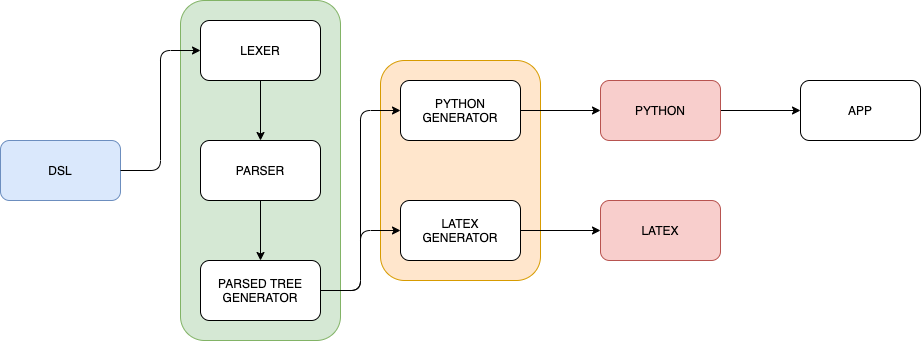
\includegraphics[width=\columnwidth]{architecture.png}
    \caption{System's architecture.}
\end{figure}

\subsection{DSL}

\subsubsection{File structure}
In our language, each file represents one and only one behavior.
A file is divided in 3 components:
\begin{itemize}
    \item \textit{Behavior} - main behavior tree;
    \item \textit{Definitions} (optional) - node definitions that can be referenced in other nodes or in the main BT;
    \item \textit{Code} - Python code where are described the execution nodes, and other code that the programmer wishes to add.
\end{itemize}

\subsubsection{Syntax}
Meter exemplo

\subsection{Compiler}
\subsubsection{Lexical analysis}
The first step in the development of a compiler is the lexical analysis, that converts a char sequence in a token sequence.
The following table shows which tokens are utilized in our compiler:
\begin{table}[H]
    \centering
    \begin{tabular}{ | p {5cm} | p {5cm} | } 
        \hline
            \multicolumn{2}{ |c| }{\textit{\textbf{Tokens}}} \\
        \hline
            \multicolumn{1}{ |c| }{\textbf{Name}} & \multicolumn{1}{ |c| }{\textbf{Value}} \\
        \hline
        \hline
            literals         & \texttt{({[]}),:\%}           \\ \hline
            RIGHTARROW       & \texttt{->}                   \\ \hline
            BEHAVIOR         & \texttt{\textbackslash bbehavior\textbackslash b}     \\ \hline
            SEQUENCE         & \texttt{\textbackslash bsequence\textbackslash b}     \\ \hline
            SELECTOR         & \texttt{\textbackslash bselector\textbackslash b}     \\ \hline
            PROBSELECTOR     & \texttt{\textbackslash bprobselector\textbackslash b} \\ \hline
            PARALLEL         & \texttt{\textbackslash bparallel\textbackslash b}     \\ \hline
            DECORATOR        & \texttt{\textbackslash bdecorator\textbackslash b}    \\ \hline
            CONDITION        & \texttt{\textbackslash bcondition\textbackslash b}    \\ \hline
            ACTION           & \texttt{\textbackslash baction\textbackslash b}       \\ \hline
            INVERTER         & \texttt{\textbackslash bINVERTER\textbackslash b}     \\ \hline
            MEMORY           & \texttt{\textbackslash bmemory\textbackslash b}       \\ \hline
            INT              & \texttt{\textbackslash d+}                            \\ \hline
            VAR              & \texttt{\$\textbackslash w+}                          \\ \hline
            NODENAME         & \texttt{\textbackslash b\textbackslash w+\textbackslash b}   \\ \hline
            CODE             & \texttt{\%\%(.|\textbackslash n)+} \\
        \hline
    \end{tabular}\\
    \caption{Lexical analysis' tokens.}
    \label{tab:tokens}
\end{table} 

\subsubsection{Syntatic analysis}
\begin{lstlisting}
    root : behavior CODE
         | behavior definitions CODE
         | definition behavior CODE

    behavior : BEHAVIOR ':' '[' node ']'

    node : SEQUENCE ':' '[' nodes ']'
         | SEQUENCE ':' VAR
         | MEMORY SEQUENCE ':' '[' nodes ']'
         | MEMORY SEQUENCE ':' VAR
         | SELECTOR ':' '[' nodes ']'
         | SELECTOR ':' VAR
         | MEMORY SELECTOR ':' '[' nodes ']'
         | MEMORY SELECTOR ':' VAR
         | PROBSELECTOR ':' '[' prob_nodes ']'
         | PROBSELECTOR ':' VAR
         | MEMORY PROBSELECTOR ':' '[' prob_nodes ']'
         | MEMORY PROBSELECTOR ':' VAR
         | PARALLEL ':' INT '[' nodes ']'
         | PARALLEL ':' VAR
         | DECORATOR ':' INVERTER '[' node ']'
         | DECORATOR ':' VAR
         | CONDITION ':' VAR
         | ACTION ':' VAR
    
    nodes : nodes ',' node
          | node
    
    prob_nodes : prob_nodes ',' prob_node
               | prob_node
    
    prob_node : VAR RIGHTARROW node

    definitions : definitions definition
               | definition

    definition : SEQUENCE NODENAME ':' '[' nodes ']'
        | SELECTOR NODENAME ':' '[' nodes ']'
        | PROBSELECTOR NODENAME ':' '[' prob_nodes ']'
        | PARALLEL NODENAME ':' INT '[' nodes ']'
        | DECORATOR NODENAME ':' INVERTER '[' node ']'
\end{lstlisting}

\subsubsection{Semantic analysis}

\section{Tools}
\label{sec:tools}

FLEX - YACC
Python
Latex

\section{Example}
\label{sec:example}


\section{Conclusion}
\label{sec:conclusion}

-- Ver com professores

\bibliography{behavior_trees}

\end{document}
